\begin{figure*}[!t]
\centering
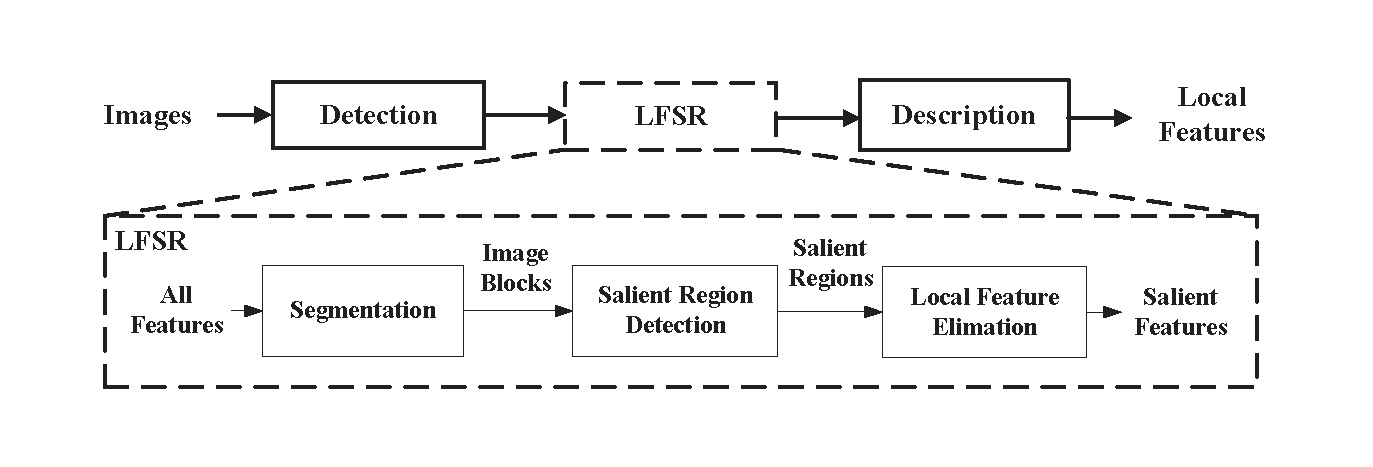
\includegraphics[width=5.0in]{images/fig-overview.eps}
\caption{An overview of Local Feature based Salient Region algorithm}
\label{fig:overview}
\end{figure*}

\section{Algorithm}
\label{sec:algorithm}

\subsection{Overview}
\label{sec:algorithm_overview}

The basic idea of LFSR is to compute salient regions for local feature reduction. Since we are not concerned with the precise region boundary in our task, it's possible to get approximate salient regions with much less computation. According to our observation, the distribution of features in one image is related to the salient region, which means most concerned local features located in one major region and other noises located apart from them with a much larger distance to the salient region center. Thus, a approximate salient region can be regarded as a region expanded from the geometry center of local features. Considering the distribution of local features in an image's x axis and y axis, the local feature based salient region should has a width and height ratio computed from the standard deviation of feature's positions on both the x axis and the y axis.

In some images with more than one major objects, there may exist several local feature dense region, result in multiple LFSR in one image. To identify and compute these scenario efficiently, we involve a preprocessing to do a simple segmentation on all local features. 

As shown in Figure \ref{fig:overview}, there exist two major stages in LFSR algorithm. 
\begin{inparaenum}[\itshape a\upshape)]
\item First, a segmentation is performed on all local features to identify whether exist multiple salient region in that image. 
\item Second, for each image segmentation, LFSR computes that segmentation's salient region individually.
\end{inparaenum}

\subsection{Local Feature Based Segmentation}
\label{sec:algorithm_segmentation}

One image may have multiple objects to construct a whole topic. When performing LFSR on this kind of images, we found that it's necessary to avoid computing the salient region across all local features in one run, which may lead to a significant precision loss.

There have been a lot of research about image segmentation, but in our research, we prefer to do a approximate segmentation only relying on the geometric meaning of local features. LFSR solve this problem by performing scan operations on both the x axis and the y axis. In each scan, a cut-point may be found following these two constraints:

\begin{enumerate}

  \item No local feature should be divided into multiple parts. Every local feature can be recognized as a dot with a radius that equals its scale and no cut-point should locate on that dot. This constraint is based on an observation that one local feature should contribute to only one object, not several objects.

  \item The cut-point should be located as near as possible to the center of image. Each scan is performed from the image center, in order to find the nearest cut-point for that image. This constraint is also based on an observation that major objects in one real photo always locate in the center, not far away from it.

\end{enumerate}

The detailed steps are shown in Figure~\ref{fig:segmentation}. The segmentation is started from the center of each axis. When a cut-point satisfying the above two constraints is found, LFSR stops scanning and takes that cut-point for the image segmentation. If a scan exceeds a threshold distance to the image center, for example $1/4$ of the image with, the scan should stop and announce that there exists no valid segmentation on that dimension. After scanning on both the x axis and the y axis, at most four image segmentations are found. If necessary, this kind of segmentation can be done recursively. But according to our observation, one run of segmentation is enough in most situations, for almost no image has more than two major objects.

\begin{figure}[!t]
\centering
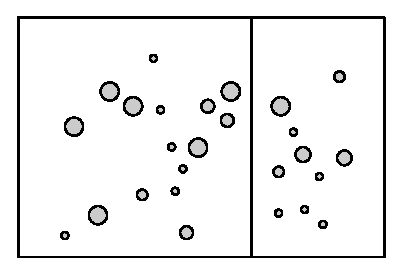
\includegraphics[width=2.5in]{images/fig-segmentation.eps}
\caption{Segmentation by scanning all local features on the x axis. The line of cut point should not go across any feature point and locate as near the image center as possible.}
\label{fig:segmentation}
\end{figure}

\begin{table*}[!t]
\begin{center}
\begin{tabular}{|l|c|c|c|c|c|}
\hline
 & Precision & Recall & F score & Reduction Efficiency & Process Time(s) \\
\hline\hline
FTSR & 0.74 & 0.59 & 0.68 & 30\% & 2828 \\
LFSR & 0.52 & 0.59 & 0.55 & 42\% & 3.2 \\
\hline
\end{tabular}
\end{center}
\caption{Comparison between FTSR and LFSR.}
\label{tab:comparison}
\end{table*}

\subsection{Local Feature Based Detection}
\label{sec:algorithm_detection}

As discussed in Section~\ref{sec:algorithm_overview}, a precise salient region detection is not necessary for local feature reduction. Thus, LFSR employs geometric meaning of local features to compute the approximate salient region.

According to Observation~\ref{itm:observation_1}, the local features of one salient region locate near to each other while noises locating far away from them. To simplify this problem, LFSR regards the geometric center of feature points as the center of salient region. Thus, the region center can be calculated like this:

{\begin{equation} \label{eq:center}
C(x, y) = \sum_{i}^{N}\left({F}_{i}(x, y) \right)
\end{equation}}

Where $C(x, y)$ means the geometric center of every local feature $F(x, y)$.

After locating the center, LFSR build the final salient region by expending the region as rectangle with a particular length-width ratio. And the ratio can also be computed directly from the distribution of features:

{\begin{equation} \label{eq:ratio}
Ratio = \sqrt{\frac{\sum_{i}^{N}\left ( x_{i}-x_{c} \right )^{2}}{\sum_{i}^{N}\left ( y_{i}-y_{c} \right )^{2}}}
\end{equation}}

Where $s_{i}$ and $y_{i}$ is every feature's position, while $x_{c}$ and $y_{c}$ is the center position computed by Equation~\ref{eq:center}. To get the final salient region, LFSR grows the region size until the amount of local feature in it exceeds a desirable number, for example 50 percent of the original local features.

Combined with segmentation discussed in Section~\ref{sec:algorithm_segmentation}, the processing result will provide several candidate regions. According to the observation \ref{itm:observation_3}, LFSR choose to eliminate regions with features fewer than a threshold $\theta$. In our evaluation, we pick up the candidate region with most local features and take $1/4$ of its local feature quantity as the threshold $\theta$.

Overall, LFSR detects the salient region with one mean value and two standard deviation computations, also with a few additional loops to expand the detected region. Since these computations are only performed on local features, the cost should be very slight when integrated with a local feature descriptor. Furthermore, we find that this simple approach also achieves an obvious performance advantage when compared to other precise salient region algorithms.